\documentclass{article}

\usepackage[english]{babel}
\usepackage{amsthm}
\usepackage{mathtools}
\usepackage{amsmath}
\usepackage{graphicx}

\newtheorem{definition}{Definition}
\newtheorem{lemma}{Lemma}
\newtheorem{theorem}{Theorem}
\newtheorem{xca}{Exercise}

\usepackage{graphicx} % Required for inserting images

\usepackage{hyperref}

\title{Graph Theory Exercises 12}
\author{Group 1: Ebba Brunvall, Anna Enerud, Ismat Halabi, \\ Victor Lemaitre and Gholam Mohammadi}
\date{December 2023}

\begin{document}

\maketitle

\section*{Exercise 1}
If the graph G has no two-connected blocks then it has no cycle which means that its components are either an isolated vertex or a tree. If G has no edge then all of its components are isolated vertices and so it has a 1-colouring. Else, as trees have a 2-colouring the graph also has a 2-colouring. 

\section*{Exercise 2}
First colour each block using at most $k = \max_{i\in[r]} \chi(B_i)$ using a different function for each block $B_i$ that we will call $c_i : B_i \rightarrow [k]$.
At each cutvertex where there is a disagreement between the colouring of an arbitrary number of different functions we will resolve the problem in the following way :
\begin{enumerate}
\item Select a block, lets call its vertices $B_x$ and call $x$ the colouring it gave to the cutvertex $c$
\item Select a block whose colouring conflicts with $B_x$, lets call it $B_y$ and call $y$ the colouring it gave to the cutvertex
\item Give $B_y$ a new colouring function  
\begin{align*} 
&c_y' : B_y \rightarrow [k] \\ 
&c_y'(v) = c_y(v) + x-y \bmod{k}
\end{align*}
this function is one to one so its still a valid colouring, furthermore we now have resolved the conflict on the cutvertex as $c_y'(c) = y + x - y = x$
\item Go back to step 2 until there is no conflict at that cutvertex
\end{enumerate}

Using that method to solve conflict and knowing that a block graph is a forest we can solve all the colouring conflicts of the graph in a simple way 
\begin{enumerate}
\item Pick a component of the block graph of G, if its a single block there is no problem thus we only consider the case where it is a tree
\item Pick a leaf of the tree, it will be a block because a cutvertex in a block graph is adjacent to two trees
\item Solve conflicts between blocks by keeping intact the colouring function of the block closest to the leaf

\end{enumerate}


For example :

      
      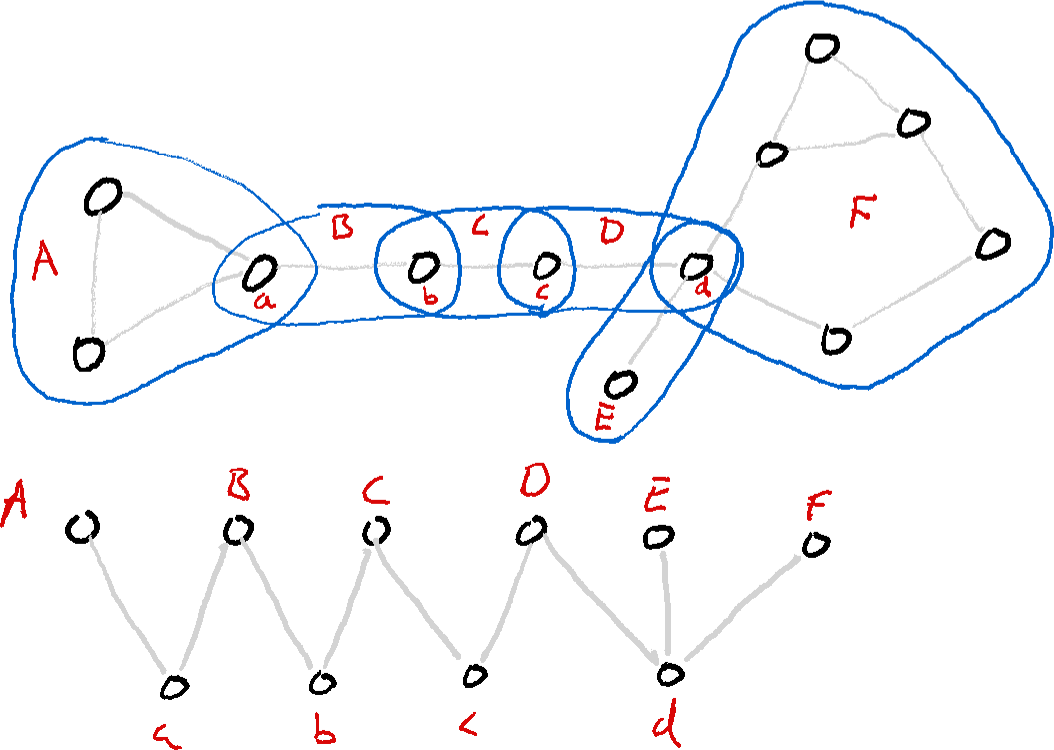
\includegraphics[width=0.9\textwidth]{graph_with_blockgraph.png}


In that block graph you would select a leaf A, E or F, let's say we pick A. Then you will change B coloring function in order to solve the possible conflict on cutvertex a, by doing that B now agrees with A on a. You repeat the process with the block C, because C is farther away from the leaf A you change C's coloring function, not B's. You repeat this process until every possible conflict of coloring on cutvertex is solved. This process is guaranteed to finish as there are no cycles on the block graph. 



\section*{Exercise 3}
 In this exercise, we use some \emph{spectral} methods for deriving results about the chromatic number. We rely on the following lemma, which can be proved using the technique of Rayleigh-quotients:

  \begin{lemma}
    Let $G$ be a graph and $H$ an induced subgraph of $G$, and let their adjacency matrices be $A_G$ and $A_H$ respectively. Then
    $$\lambda_{\min}\left(A_G\right) \leq \lambda_{\min}\left(A_H\right) \leq \lambda_{\max}\left(A_H\right) \leq \lambda_{\max}\left(A_G\right),$$
    and
    $$\delta(G) \leq \lambda_{\max}\left(A_G\right) \leq \Delta(G),$$
    where $\delta(G)$ and $\Delta(G)$ are the minimum and maximum degree of $G$.
  \end{lemma}

  Use the above lemma to prove the below theorem:
  \begin{theorem}[Wilf, 1967]
    For any graph $G$ with adjacency matrix $A_G$, we have
    $$\chi(G) \leq \lambda_{\max}\left(A_G\right) + 1.$$
  \end{theorem}

  \textbf{Hint:} Let $H$ be a minimal induced subgraph of $G$ with $\chi(H) = \chi(G)$. Can you relate the minimum degree of $H$ to the chromatic number of $G$?
  
\paragraph{Solution from earlier lecture notes:} Among all induced subgraphs of $G$ there exists a minimal subgraph $H$ (w.r.t inclusion) with $\chi(H)= \chi(G)$. Let $v$ be a vertex of $H$. Then $H - \{v\}$ admits a $\chi(G) - 1$- colouring, and if $deg_{H}(v) < \chi(G) - 1$. then this colouring could be extended to a $\chi(G) - 1$-colouring of $H$, contradicting our choice of $H$. Hence, the minmium degree in $H$ is at least $\chi(G) - 1$. Denote by $A_{H}$ the adjacency matrix of $H$. Then, 
$$\chi(G) \leq \delta(H) + 1 \leq \lambda_{max}(A_{H}) + 1\leq \lambda_{max}(A_{G}) + 1$$ where we used the inequalities from Lemma 1.\\

We also present a solution that is a bit longer but at least not stolen from the earlier lecture notes:

\paragraph{Alternative solution:} Using the hint we let $H$ be a minimal induced subgraph of $G$ with $\chi(H) = \chi(G)$. (Such an induced subgraph always exists) 

\paragraph{\underline{Claim:}} $\chi(G) \leq \delta(H) + 1 $ 

\paragraph{} Since $H$ is minimal, it is of size $\chi(G)$. To prove the claim we do induction in the size of $G$. For this we assume that $G$ is always coloured with the minimal amount of colours and that we don't remove any edges from $G$. 

\paragraph{\underline{Base case:}} 
$|G|=1$. Then $\chi(G) = 1$ and $\delta(H) = \delta(G) = 0  \Rightarrow \chi(G) = 1 = \delta(H) + 1$ and so the claim holds for the base case.

\paragraph{\underline{Induction assumption:}} Assume the claim holds when $|G| = n$ and $\chi(G) = k$

\paragraph{\underline{Induction step:}} 
Now $|G| = n+1$ and we get two cases:

\begin{enumerate}
    \item \underline{No new colour is added:} Then $\chi(G) = k$ still and since we didn't remove any edges: $\chi(G) = k \leq \delta(H) + 1$ by the inductive assumption.
    \item \underline{One new colour is added:} We have now added a new vertex and edges s.t $\chi(G) = k+1$.
    Since $\chi(G) = \chi(H)$ this vertex must have also been added to $H$, we call this vertex $v$. By the definition of a k-colouring, $v$ must have at least degree $k$ since it must be adjacent to at least one of every previously used colour. This gives two cases:
    
\begin{enumerate}
    \item $d_{v} = \delta(H) \geq k$ i.e $v$ is the vertex with lowest degree in $H$. Then $\chi(G) = k+1 \leq \delta(H) + 1$ and so the claim holds. Note that this is only the case when the graph is regular, since otherwise there would be at least one other vertex with degree larger than $k$ and then $\chi(G) > k+1$
    
    \item $d_{v} \neq \delta(H)$ i.e one of the "old" vertices, say $u$, has the minimum degree. By the inductive assumption $k \leq \delta(H \setminus \{v\}) + 1$ so for $k+1 \leq \delta(H) +1$ to hold we need that $\delta(H \setminus \{v\}) + 1 \leq \delta(H)$ i.e we need that the new vertex $v$ is adjacent to $u$. Note that $| H | \geq \chi(G)$ since otherwise our construction of $H$ would be contradicted ($\chi(G) = \chi(H) = k+1$ cannot hold if $H$ does not have at least $k+1$ vertices). This means that $u$ must be adjacent to $v$ in $H$ since otherwise we could have used $u's$ colour for $v$ (in $H$) if so $\chi(H) $ would not equal $ \chi(G)$ which contradicts our construction. Remember here that $H$ is minimal! Otherwise there could be another vertex with $u's$ colour that could be adjacent to $v$. This gives that $\delta(H) = d_{u} \geq \delta(H \setminus \{v\}) +1  \Rightarrow  \chi(G) = k+1 \leq \delta(H) +1$
\end{enumerate}
\end{enumerate}

So then the claim that $\chi(G) \leq \delta(H) + 1$ holds and by lemma 1: $$\chi(G) \leq \delta(H) + 1 \leq \lambda_{max}(A_{H}) + 1 \leq \lambda_{max}(A_{G}) + 1$$
Which is what we wanted.

\section*{Exercise 4 (Extra)}
Assume you have to separate English alphabet letters into boxes such that no two consecutive letters end up in the same box. What is the minimum number of boxes you need for this task?

\noindent
(Source: \url {https://math.libretexts.org/Courses/Saint_Mary%27s_College_Notre_Dame_IN/SMC:_MATH_339_-_Discrete_Mathematics_%28Rohatgi%29/Text/5:_Graph_Theory/5.E:_Graph_Theory_%28Exercises%29})

\paragraph{Solution:}
If we transform the problem into a graph where each letter is a vertex and vertices represent consecutive edges, we will have a graph with degree 1 (letters A and Z) and 2 (other letters). By Brook's theorem, this graph has $\chi(G) = 2$ and the graph is not complete nor has odd cycles. Hence, it is enough with two boxes only.

\section*{Exercise 5 (Extra)}
Prove that if a graph has at most two cycles of odd length then it can be
coloured with 3 colours. \textit{Hint}: a bipartite graph has $\chi(G) = 2$.

\paragraph{Solution:}
(Based on University of Victoria course notes in Discrete and Combinatorial Mathematics).\\

\noindent
We must consider three distinct cases.\\

\noindent
Case 1: Suppose G has no odd cycles. Then G is bipartite with $\chi(G) = 2$, so
certainly we can colour G with three colours.\\

\noindent
Case 2: Suppose that G contains exactly one odd cycle, C. Then certainly
$\chi(G) > 2$ as this graph is not bipartite. Consider removing an arbitrary vertex
u $\in$ C from G, this would create a graph with no odd cycles. So, G - u is
2-colourable. Adding u back to G would only require one additional colour, so G is 3-colourable.\\

\noindent
Case 3: Suppose G contains exactly two odd cycles, $C_1$ and $C_2$, we now consider
two subcases:\\

Case 3a: Suppose that $C_1$ and $C_2$ share a common vertex, u. Consider
G-u, which now has no odd cycles since removing a vertex from
a cycle breaks the cycle. Thus, G - u is bipartite and 2-colourable.
Adding back u will require at most one additional colour, so G is
3-colourable.\\

Case 3b: Suppose $C_1$ and $C_2$ share no common vertices. If every
vertex in $C_1$ is adjacent to every vertex in $C_2$ then there would be
another odd cycle in G which is impossible by assumption. Thus,
there exists two vertices, u $\in C_1$ and v $\in C_2$, such that uv $\notin$ E(G).
Consider obtaining the graph G - u - v, this will break both cycles
in G, making G - u - v a graph free of odd cycles, and hence
2-colourable. As u and v are not adjacent in G colouring them will
require at most one additional colour. Thus, G is 3-colourable.\\

\noindent
This completes the proof.
\end{document}
